\section{Results}

\subsection{Position matters, without making length irrelevant}

In documented means, moving a 30-day gap from zero to full climatological overlap raises climatology H30 absolute error by \RPosition{}\,$^{\circ}$C [\RPositionLow{}, \RPositionHigh{}] (Figure~\ref{fig:recovery}). The broadened and warm-season controls show that this is not confined to the earlier small provider subset. Its magnitude nevertheless depends on reconstruction and auxiliary information (SI Tables S4--S6).

Length retains an effect. Where the true peak is entirely hidden, extending 30 to 90 days raises climatology error by \RLength{}\,$^{\circ}$C [\RLengthLow{}, \RLengthHigh{}], and interpolation error by \RInterpLength{}\,$^{\circ}$C [\RInterpLengthLow{}, \RInterpLengthHigh{}]. Fragmentation changes true support exposure despite equal total warm missing days. These contrasts do not support an assertion that only peak-window hiding damages H30, or that length and method rankings are invariant. Target-aware assessment is warranted; one overlap number is not a sufficient replacement for completeness information.

\begin{figure}
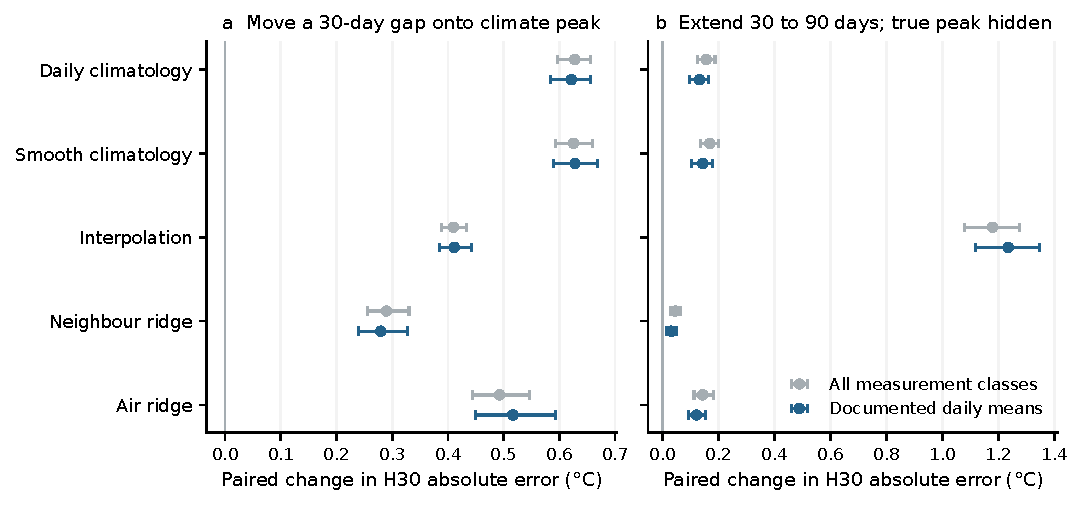
\includegraphics[width=\textwidth]{figures/r3_f1_recovery.pdf}
\caption{Paired mechanism contrasts. (a) Full-minus-zero climatological overlap for equal 30-day gaps. (b) Extension from 30 to 90 days with the true peak entirely hidden. Blue denotes documented daily means, gray all measurement classes; bars are component-bootstrap intervals. Starts are averaged within station-years, not counted as independent rivers.}
\label{fig:recovery}
\end{figure}

\subsection{An identity does not itself identify a deployable remedy}

The identity holds to numerical precision and the switch increment is nonnegative (SI Table S7). Among positive climatology increments, \RCompensatingSwitchShare{}\% still end below true H30. Switching often buffers cold errors rather than fabricating hot extremes (Figure~\ref{fig:channels}).

Climatology oracle mean absolute errors are \ROracleRaw{}\,$^{\circ}$C originally, \ROraclePermuted{} after permutation, \ROracleDemeaned{} after centering and \ROracleBoth{} after both. The interaction is \ROracleInteraction{}\,$^{\circ}$C, so improvement percentages are not additive mechanism shares. The visible-information correction improves policy MAE by only \RDeployableImprovement{}\,$^{\circ}$C [\RDeployableLow{}, \RDeployableHigh{}]. The oracle diagnoses structure without demonstrating a large available correction.

\begin{figure}
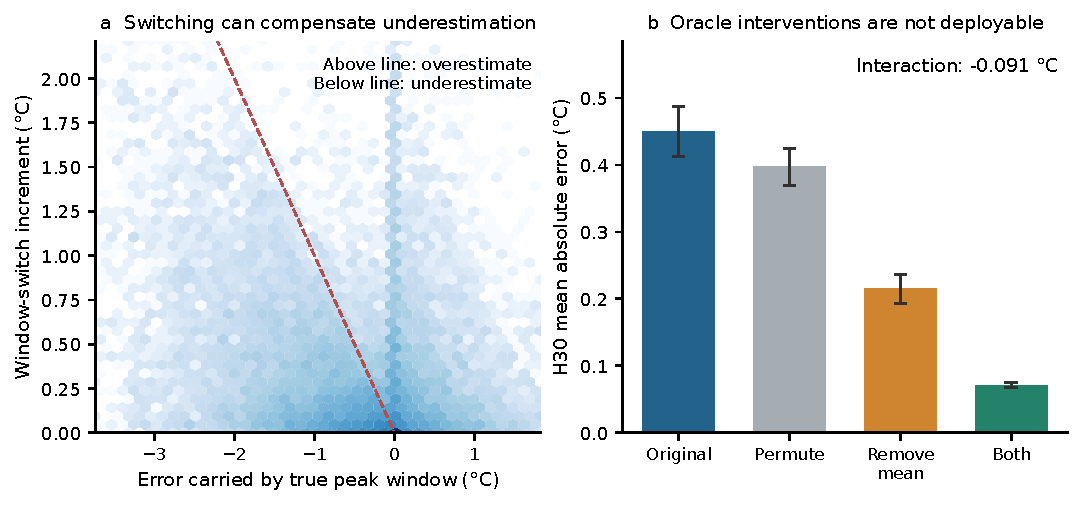
\includegraphics[width=\textwidth]{figures/r3_f2_channels.pdf}
\caption{Error structure and operational limits. (a) Climatology true-window error versus switch increment in documented-mean, replicate-zero controlled masks. The diagonal separates net under- and overestimation; axes show the central 99\% range. (b) Truth-dependent factorial interventions with component-bootstrap intervals. Their interaction is nonzero. The small deployable improvement is reported separately, not inferred from these bars.}
\label{fig:channels}
\end{figure}

\subsection{Direct target uncertainty explains the representation's gain}

On the admission mixture, uncertain-window source retention improves over the matched H30-generic score by \RRetGainMin{}--\RRetGainMax{} points across seeds, not the predefined five-point practical gain (Figure~\ref{fig:information}). Earlier-years-only \emph{local-input} comparisons give \RPriorLocalGainMin{}--\RPriorLocalGainMax{} points, but are not a global forward pipeline. In the fully refitted calendar-time forward experiment, the mean difference is \RWholePriorGain{} points with whole-procedure interval [\RWholePriorLow{}, \RWholePriorHigh{}]. Retrospective whole-procedure uncertainty is also broad: \RWholeRetGain{} [\RWholeRetLow{}, \RWholeRetHigh{}].

Direct H30 uncertainty gives essentially the same conditional source retention as the larger window representation. Their conditional paired intervals lie within the predefined two-point equivalence band, whereas whole-procedure intervals do not establish equivalence. Complete historical diagnostics are also competitive. This distinguishes target-specific diagnostics from a necessary uncertain-window representation, not models with and without all peak information. Small-model support features, flexible seasonal alternatives, daily-versus-H30 disagreement and component removals appear together (SI Tables S9--S13), rather than selecting a favorable ablation.

Target awareness nevertheless has identifiable value. Replacing daily disagreement with H30 disagreement improves source retention by \RTargetDailyMin{}--\RTargetDailyMax{} points with matched learner and reconstruction information. On independent Swiss records after local recalibration, the difference is \RTestRetTargetDailyGain{} points [\RTestRetTargetDailyLow{}, \RTestRetTargetDailyHigh{}]. Explicit overlap adds \RSmallSupportMin{}--\RSmallSupportMax{} points to the small logistic model, but its increment to the seasonal spline ranges from \RSplineSupportMin{} to \RSplineSupportMax{} points. H1 therefore supports target-specific diagnosis, not a universally necessary overlap variable or a demonstrated small-data advantage over flexible seasonal representations.

The trajectory scores are not calibrated probabilities. Raw 90\% scenario-band coverage is only \RBandSwissRet{}\% in retrospective Swiss admission and \RBandSwissPrior{}\% prospectively. Their representation comparison does not establish that a better joint predictive distribution could never make window information useful.

\begin{figure}
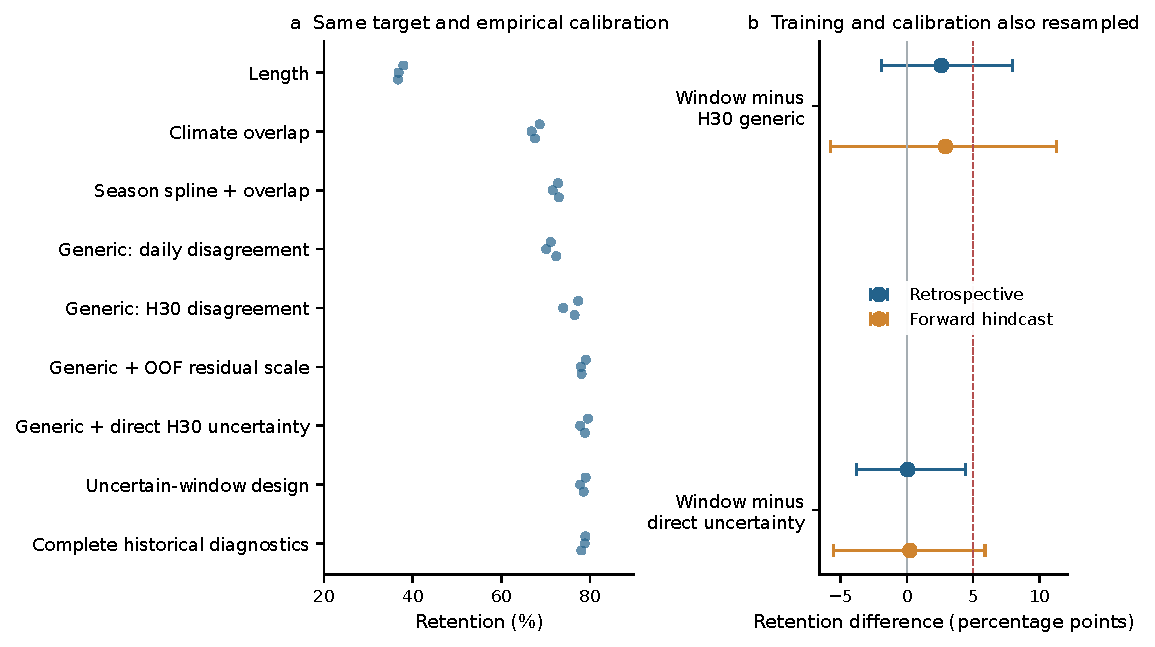
\includegraphics[width=\textwidth]{figures/r3_f3_information.pdf}
\caption{Contribution attribution on the admission cohort. (a) Retention under the common empirical calibration target; each dot is a split sensitivity, not independent replication. OOF denotes out-of-fold residuals of the actual reconstructor. (b) Whole-procedure intervals refit learning and calibration and resample evaluation components. The dashed line is the five-point superiority margin. Small conditional differences do not imply whole-procedure equivalence.}
\label{fig:information}
\end{figure}

\subsection{Independent transfer does not establish its calibration target}

On \RTestRetCases{} Swiss documented-mean cases from \RNewSwissTest{} held-out components, uncertain-window F0 retains \RTestRetFrozenRetention{}\% with \RTestRetFrozenRisk{}\% failures (Figure~\ref{fig:transfer}). Unchanged transfer therefore misses the nominal 5\% target at its observed operating point. Seven-component intervals do not establish that population risk is strictly above 5\%; they also do not validate a transferable guarantee. Local recalibration gives \RTestRetRecalibratedRetention{}\% retention and \RTestRetRecalibratedRisk{}\% point risk; local fitting gives \RTestRetLocalRetention{}\% and \RTestRetLocalRisk{}\%. Neither lower point risk nor zero observed failures proves a network guarantee.

The calendar-time forward Swiss pool is smaller, \RTestPriorCases{} cases. Unchanged-transfer retention and risk are \RTestPriorFrozenRetention{}\% and \RTestPriorFrozenRisk{}\%; recalibration gives \RTestPriorRecalibratedRetention{}\% and \RTestPriorRecalibratedRisk{}\%. French aggregates, unseen-provider and intercontinental transfers, joint certificate delivery and complete diagnostics are separate (SI Table S14). They do not supply the missing independent five-point, common-risk representation advantage. H2 is not supported.

Reconstruction remains consequential. Across both new measurement scopes on matched forcing-supported controlled cases, Air2stream-3 has MAE \RPhysicalThreeMAE{}\,$^{\circ}$C versus \RPhysicalThreePolicyMAE{} for the fixed policy. Air2stream-8 has \RPhysicalEightMAE{} versus \RPhysicalEightPolicyMAE{} on \RPhysicalEightCases{} cases, but additionally uses discharge. These are not pure architectural comparisons, nor an end-to-end admission advantage: the process references were not substituted into the frozen risk training. The common priority point defines a controlled comparison object, not the best attainable reconstruction under every input budget.

Constructed rare-group and correlated-failure experiments show why empirical calibration is not generally conservative (SI Table S18). The rigorous rule cannot certify nonzero admission with available evidence. Component counts and corrected hydrological, anomaly and event strata expose uncertainty hidden by pooled percentages (SI Tables S15--S17). Event/cofailure tests are nondegenerate on held-out opened-source networks, not independent target confirmation (SI Figure S2).

\begin{figure}
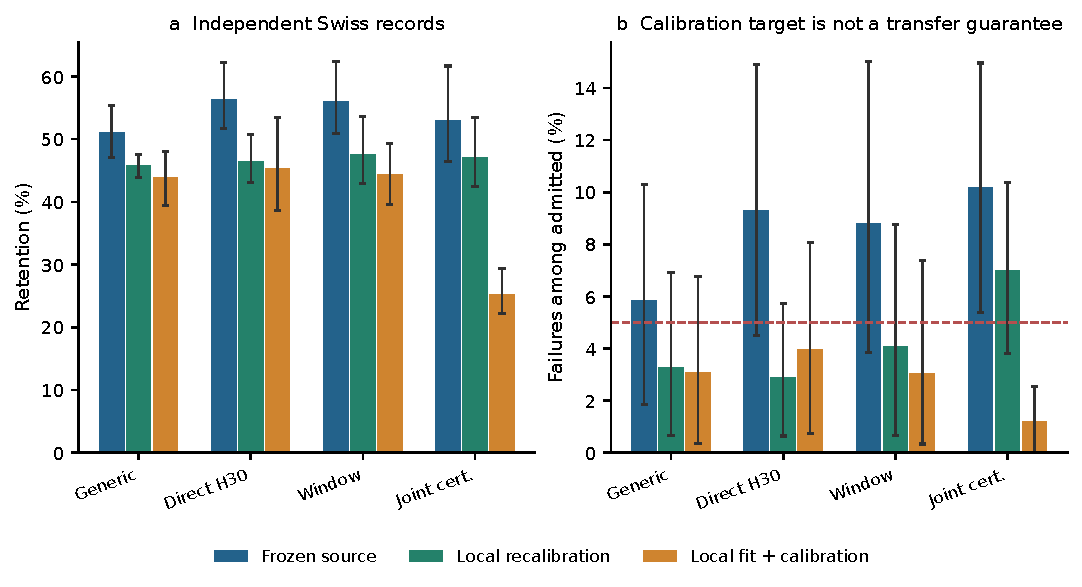
\includegraphics[width=\textwidth]{figures/r3_f4_transfer.pdf}
\caption{Independent Swiss transfer. Source model and threshold are frozen in F0; only target calibration changes in F1; F2 fits on new development stations and calibrates locally. The joint certificate chooses its own reconstruction; other arms deliver the common point. Bars show descriptive test-component bootstrap uncertainty, not distribution-free guarantees. The horizontal calibration target is exceeded after unchanged transfer.}
\label{fig:transfer}
\end{figure}

\subsection{Refusal has a use-dependent benefit and an information cost}

For locally hot-year classification, Swiss F0 refuses \RTestRetHotRefusal{}\% of true hot cases, \RTestRetCoolRefusal{}\% of cool cases and \RTestRetOverallRefusal{}\% overall. The earlier opened-panel statement that hot years are not disproportionately refused is not a universal property. Refusal changes both the judged sample and unknown fraction (Figure~\ref{fig:utility}; SI Table S24).

At missed-hot cost five and unknown-answer cost 0.05 relative to a false-hot answer, loss changes by \RTestRetMagnitudeLossDifference{} per original candidate [\RTestRetMagnitudeLossLow{}, \RTestRetMagnitudeLossHigh{}] versus reconstructing all. This is not sufficient to justify the selective policy: its absolute loss is \RTestRetMagnitudeAbsoluteLoss{}, whereas declaring every record unknown costs only 0.05. We added this deterministic comparator in a post-test audit without changing predictions or the predefined cost grid (SI Table S23). Some other declared cells beat both fixed alternatives at their point estimates, not under a simultaneous or measured management-utility guarantee. With inexpensive errors and costly abstention, even the reconstruct-all comparison can reverse. Observed-hot rescue adds only \RTestRetJudgementRescued{} labels here and \RTestPriorJudgementRescued{} prospectively. H3 holds only for its specified reconstruct-all scenario comparison, not a generally superior operational policy.

Recorded-calendar replay limits a benign-outage interpretation too. New eligible calendars are French aggregates, not Swiss documented-mean confirmation. Across \RNaturalCases{} masks in \RNaturalGroups{} components, unscreened failure is \RNaturalObservedRisk{}\%; the source-fitted composition rule predicts \RNaturalPredictedRisk{}\%. These are conditional replay risks, not error prevalence across complete and incomplete monitoring years combined. They neither reproduce the earlier small replay's benign average nor justify a claim that most networks need no screen. Single-network advice and source-only prediction intervals are not certification (SI Table S20).

\begin{figure}
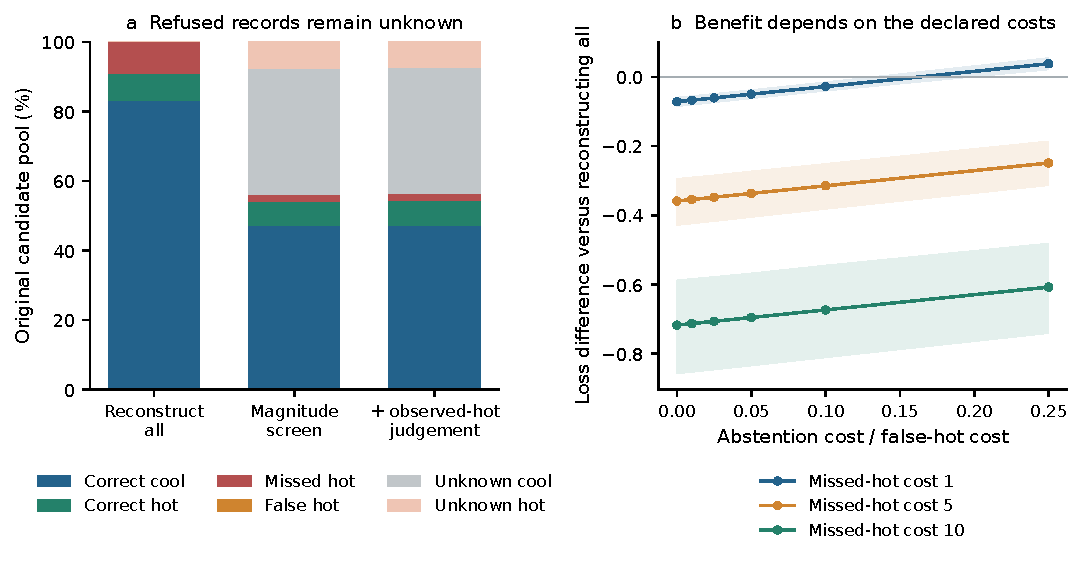
\includegraphics[width=\textwidth]{figures/r3_f5_utility.pdf}
\caption{Original-candidate downstream closure for the frozen Swiss policy and local hot threshold. (a) Correct, mistaken and unknown outcomes retain their denominator. Unknown hot/cool categories use reference truth for evaluation only. (b) Loss differences under declared costs; negative favors screening. Shading is descriptive conditional uncertainty, not simultaneous inference over the grid or a measured valuation of monitoring decisions.}
\label{fig:utility}
\end{figure}

